\chapter{Introduction}

I will show how we did hierarchical modelling of stars.

\section{Hierarchical Bayesian Models}

NEEDS INTRODUCING AND REMEMBER THE AUDIENCE. TURN PACKED SENTANCES INTO PARAGRAPHS TO GUIDE THE READER THROUGH.

Consider a model for a single object comprising a set of independent parameters, $\bm{\theta} = \{\theta_i\}_{i=1}^{N_\theta}$ which makes a set of predictions, $\bm{\mu}_y = \{\mu_{y,\,j}\}_{j=1}^{N_y}$ where $\bm{\mu}_y = \bm{f} (\bm{\theta})$. Using Bayes' theorem, we may write the \emph{posterior} probability density function (PDF) of the model given a set of observations $\bm{y}$ as,
%
\begin{equation}
    p(\bm{\theta}|\bm{y}) = \frac{p(\bm{y}|\bm{\theta})\,p(\bm{\theta})}{p(\bm{y})},
    \label{eq:bayes}
\end{equation}
%
where $p(\bm{y}|\bm{\theta})$ is the \emph{likelihood} of the data given the model, $p(\bm{\theta})$ is the \emph{a priori} PDF of the model parameters, and $p(\bm{y})$ is the \emph{evidence} of the data. 

Assuming our observations of $\bm{y}$ are uncorrelated and subjected to random, Gaussian noise with a known standard deviation, $\bm{\sigma}_y$, we may write the likelihood function as a normal distribution,
%
\begin{align}
    p(\bm{y}|\bm{\theta}) = &\prod_{j=1}^{N_y} \frac{1}{\sigma_{y,\,j} \sqrt{2\pi}} \exp \left[ - \frac{(y_j - \mu_{y,\,j})^2}{2 \sigma_{y,\,j}^2} \right],\\
    \equiv &\prod_{j=1}^{N_y} \mathcal{N}(y_j | \mu_{y,\,j}, \sigma_{y,\,j}).
\end{align}
%

The prior PDF of the model, assuming the parameters are independent, is $p(\bm{\theta}) = \prod_i p(\theta_i)$. Encoding our prior understanding of the model this way is useful for improving our inference. For example, we have independent evidence that the age of the universe is $\sim \SI{14}{\giga\year}$ [CITE]. Hence, we may choose to give the age parameter for a stellar model a uniform prior PDF from \SIrange{0}{14}{\giga\year} such that our posterior PDF is not influenced by unphysical ages.

The evidence is the PDF of the observational data. We write this as the normalisation of the numerator of Equation \ref{eq:bayes},
%
\begin{equation}
    p(\bm{y}) = \int_{-\infty}^{+\infty} p(\bm{y}|\bm{\theta})\,p(\bm{\theta})\,\dd \bm{\theta}.
\end{equation}
%

There are many ways to determine the posterior PDF, either analytically or numerically using e.g. Markov chain Monte Carlo (MCMC) through algorithms such as Metropolis-Hastings and Hamiltonian Monte-Carlo (HMC) [CITE]. Once we have the posterior, we can determine the marginalised posterior distribution of an individual parameter by integrating over all other parameters. For example, the marginalised posterior for $\theta_1$ is,
%
\begin{equation}
    p(\theta_1 | \bm{y}) = \int_{-\infty}^{+\infty} p(\bm{\theta} | \bm{y}) \, \dd \theta_2 \dots \dd \theta_{N_{\theta}}.
\end{equation}
%
Therefore, we end up with a distribution which describes the probability of $\theta_1$ given $\bm{y}$ which takes into account the distribution (or uncertainty) of all other parameters in the model.

The model described above can be applied to a single object such as a star. Let us now consider modelling a population of $N_\mathrm{obj}$ similar objects. We could combine the posteriors for each object to get a posterior for the population of objects,
%
\begin{equation}
    p(\bm{\Theta}|\bm{Y}) = \prod_{k=1}^{N_\mathrm{obj}} p(\bm{\theta}_k|\bm{y}_k),
\end{equation}
%
where $\bm{\Theta} = \{\bm{\theta}_k\}_{k=1}^{N_\mathrm{obj}}$ and $\bm{Y} = \{\bm{y}_k\}_{k=1}^{N_\mathrm{obj}}$ are the matrices of model parameters and observations. We refer to this as a \emph{no-pooled} model because no information is shared between the objects. However, what if we have a model which describes the distribution of a particular $\bm{\theta}_i$ in the population? For example, if all the objects are stars in an open cluster which formed at roughly the same time, such as Messier 67 [CITE], we might want to encode such information into the model. One method would be to independently model the stars in the cluster and then find their population mean and standard deviation in age. It has been shown that this method typically over-predicts the standard deviation because it propagates the object-level uncertainties [CITE]. Alternatively, we can incorporate the assumption that stars in a cluster formed at the same time using one of two ways. The first is to \emph{partially-pool} and the second is to \emph{max-pool} the stellar ages respectively. The former assumes the object-level parameters are drawn from some common distribution, and the latter is the special case where all object-level parameters share the same value in the population.

We refer to models which pool parameters in this way as hierarachical models [CITE]. We describe the distribution of $\bm{\Theta}$ in the population by a set of \emph{hyper-parameters}, $\bm{\phi} = \{ \phi_l \}_{l=1}^{N_\phi}$. Bayes' equation now becomes,
%
\begin{equation}
    p(\bm{\phi}, \bm{\Theta} | \bm{Y}) = \frac{p(\bm{Y} | \bm{\Theta}) \, p(\bm{\Theta} | \bm{\phi}) \, p(\bm{\phi})}{p(\bm{Y})}
\end{equation}
%
where the probability of $\bm{\Theta}$ given $\bm{\phi}$ is,
%
\begin{equation}
    p(\bm{\Theta} | \bm{\phi}) = \prod_{k=1}^{N_\mathrm{obj}} d(\bm{\theta}_k | \bm{\phi}),
\end{equation}
%
and $d(\bm{\theta}_k | \bm{\phi})$ is some chosen distribution from which the parameters for a given object are drawn from the population.

Let us consider a simple model which predicts the luminosities, $\bm{L}$ from the ages, $\bm{\tau}$ of $N_\mathrm{obj} = 1000$ stars in a cluster formed at roughly the same time. Modelling the population independently, we get the posterior,
%
\begin{equation}
    p(\bm{\tau} | \bm{L}) \propto \prod_{k=1}^{1000} p(L_k | \tau_k) \, p(\tau_k).
    \label{eq:age-np}
\end{equation}
%
Now, let us consider a partially-pooled model where the stellar ages are drawn from a normal distribution centred on a mean, $\mu_\tau$ and standard deviation, $\sigma_\tau$. The posterior now becomes,
%
\begin{equation}
    p(\mu_\tau, \sigma_\tau, \bm{\tau} | \bm{L}) \propto p(\bm{L} | \bm{\tau}) \, p(\bm{\tau} | \mu_\tau, \sigma_\tau) \, p(\mu_\tau, \sigma_\tau),
    \label{eq:age-pp}
\end{equation}
%
where,
%
\begin{equation}
    p(\bm{\tau} | \mu_\tau, \sigma_\tau) = \prod_{k=1}^{1000} \mathcal{N}(\tau_k | \mu_\tau, \sigma_\tau).
\end{equation}

There is no known analytical or empirical relation between the age of a star and its luminosity, but for the purposes of this example let us say that we know $L \propto \tau^{2}$. I generated 1000 stellar ages from a normal distribution with a mean of \SI{5}{\giga\year} and a standard deviation of \SI{0.05}{\giga\year}, and computed their luminosities using this relation. Then, I added Gaussian noise to the luminosities with a standard deviation of \SI{0.05}{\solarluminosity} and proceeded to model the stellar ages using Equations \ref{eq:age-np} and \ref{eq:age-pp} and the Bayesian package \texttt{pymc3} [CITE]. The observed and true luminosities are plot against the true ages in Figure \ref{fig:obs_lum} to show

\begin{figure}[t]
    \centering
    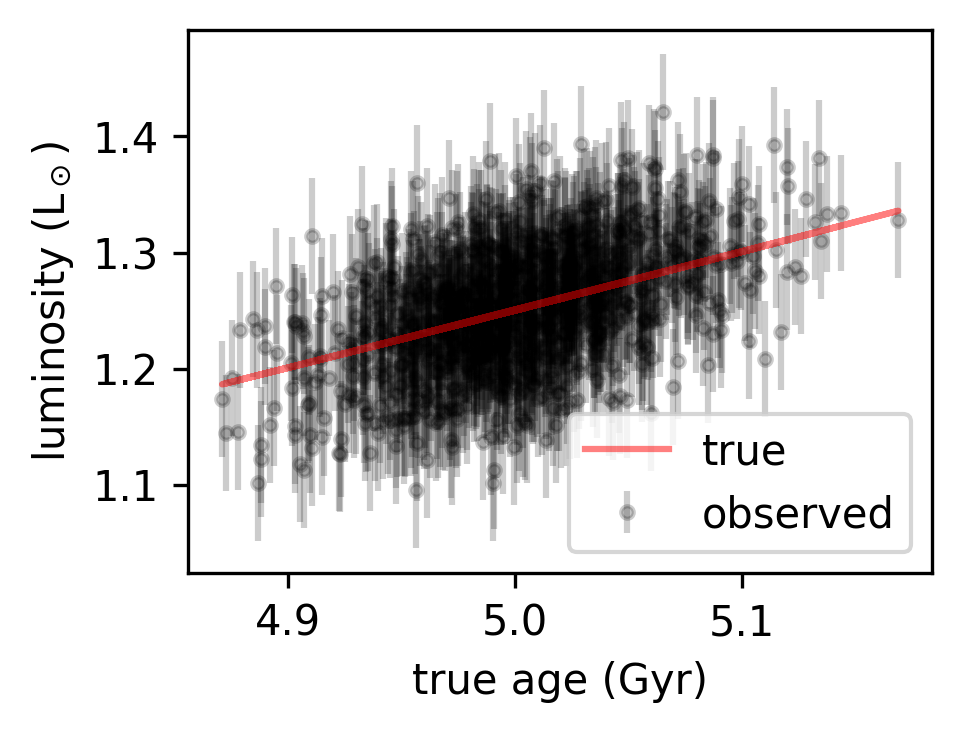
\includegraphics[]{introduction/images/obs_lum.png}
    \caption{Luminosity against true ages of a fake stellar cluster. The true luminosities lie on the red line and the observed luminosities (black) have been artificially scattered by \SI{0.05}{\solarluminosity}.}
    \label{fig:obs_lum}
\end{figure}

If we wished to determine spread of stellar ages in the cluster using the no-pooled model, we might na\"{i}vely calculate a standard deviation from the resulting stellar ages. However, this overestimates the true standard deviation, getting \SI{0.109}{\giga\year} rather than \SI{0.05}{\giga\year}, because it includes the uncertainty in the individual ages. When we model the population mean and spread in the hierarchical model we get $\mu_\tau = \SI{5.002(3)}{\giga\year}$ and $\sigma_\tau = \SI{0.042(7)}{\giga\year}$ which are within $< 2\sigma$ of the truths. Therefore, the hierarachical model is a better way of determining population-level statistics than the traditional no-pooled model.

Both models can accurately determine ages, but the hierarchical model returns more precise ages, assuming our prior assumptions are true. Figure \ref{fig:zscore} shows that the $z$-score for ages from both models match a normal distribution with a mean of 0 and standard deviation of 1, indicating the individual stellar ages and uncertainties are accurate. However, the partially pooled model produces more than doubly precise ages, as shown in Figure \ref{fig:age_unc}, because the model takes into account the population mean and spread as hyper-parameters. The reduced scatter on stellar ages is also reflected in the top-left plot of Figure \ref{fig:zscore}.

\begin{figure}[t]
    \centering
    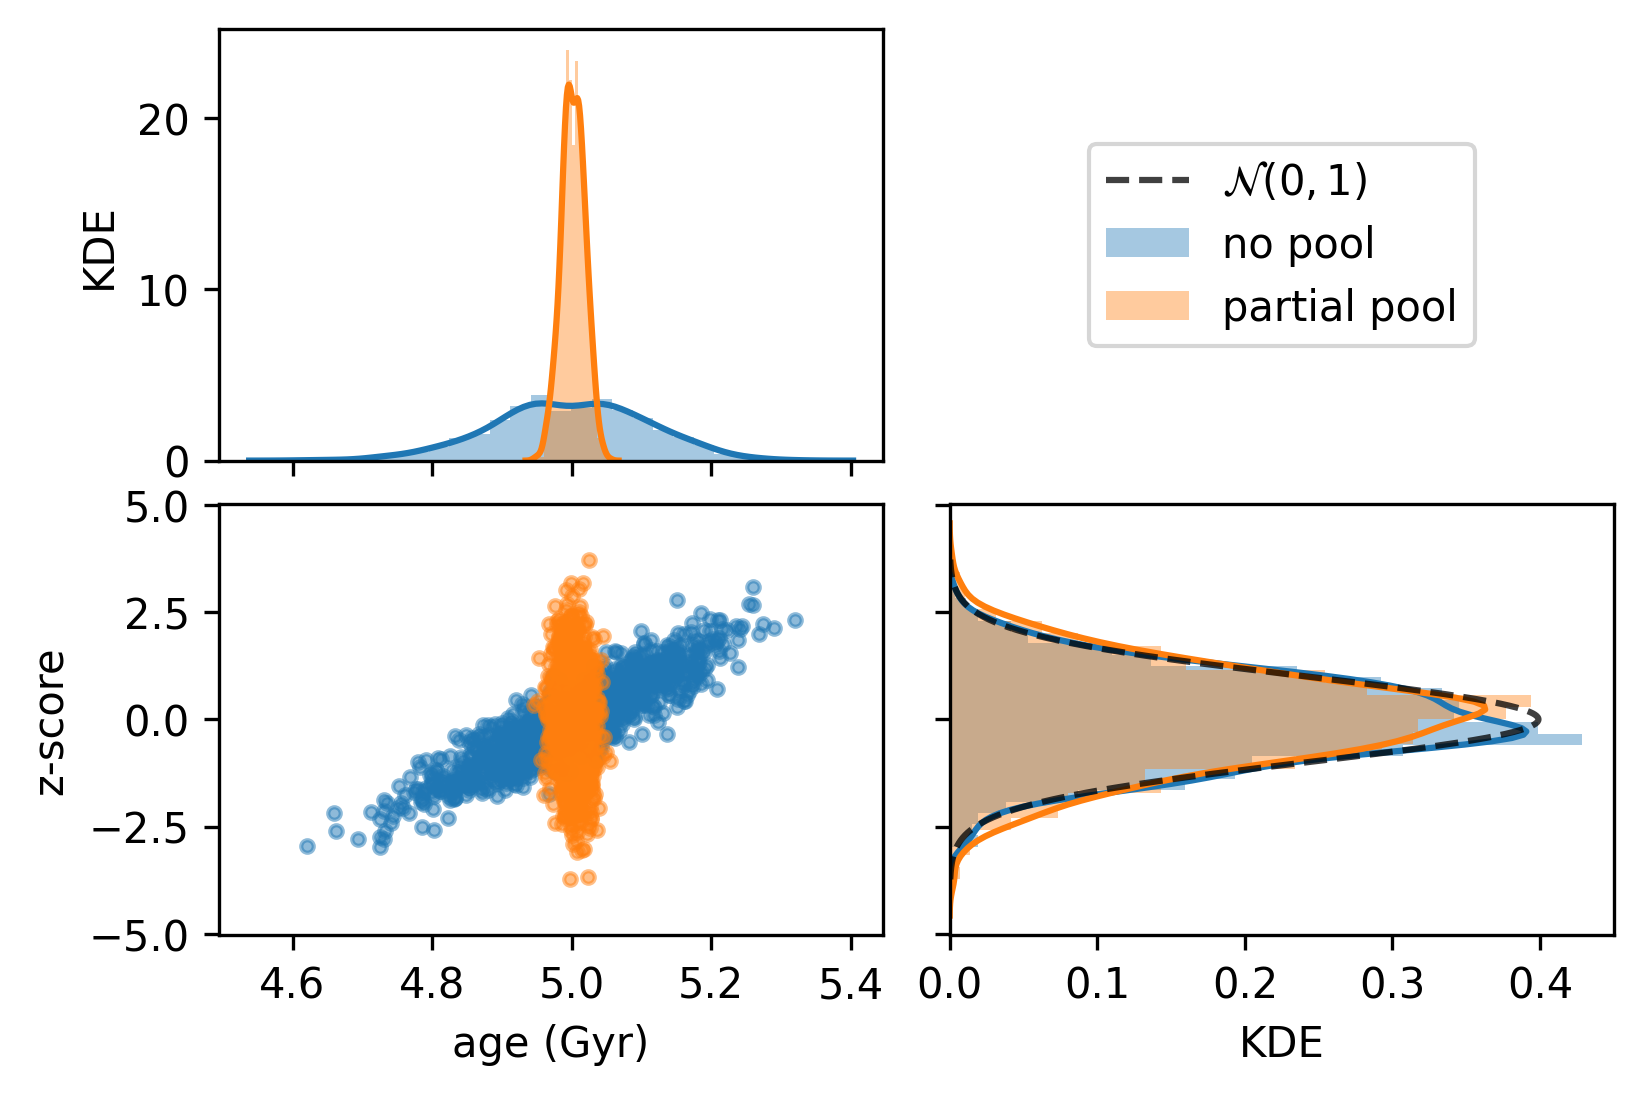
\includegraphics[]{introduction/images/age_z_score.png}
    \caption{The $z$-score, $(\bar{\tau} - \tau_\mathrm{true}) / s_\tau$, where $\bar{\tau}$ and $s_\tau$ are the respective sample mean and standard deviation of the posterior ages from each of the no- and partially-pooled models.}
    \label{fig:zscore}
\end{figure}

\begin{figure}[t]
    \centering
    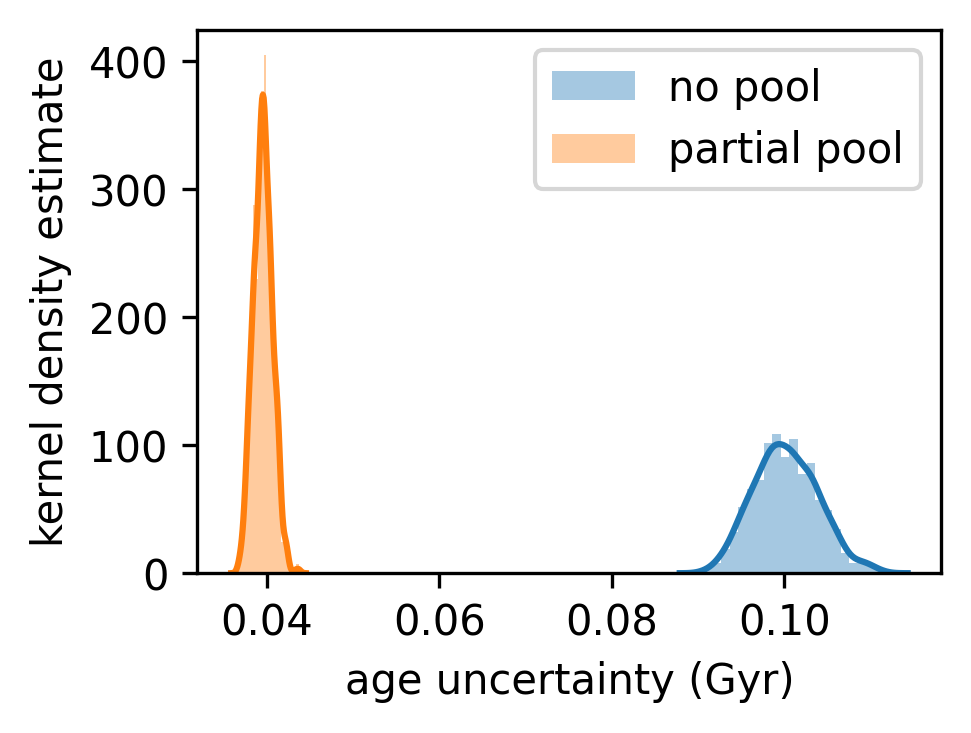
\includegraphics[]{introduction/images/age_uncertainties.png}
    \caption{Standard deviations, $s_\tau$ of the age posteriors from both the no- and partially-pooled models.}
    \label{fig:age_unc}
\end{figure}

If we wish to improve the precision of fundamental stellar parameters, using hierarchical models to encode our prior knowledge is essential. However, modelling stars is not as simple, nor analytical as in the example above. Before we can statistically model a population of stars, we must have a way of generating stellar observables from fundamental parameters such as age and mass. In the next section, I give an overview of how we numerically model stellar observables and why traditional methods pose new problems when adapting the above model.

\section{Modelling a Star}

How do we model stellar observables? A bit of history of the topic including \citet{Eddington1926}. Then Chandrasekhar 1939 and Schwartzschild 1958.

Introduction of stellar computational codes in the 1960s e.g. Iben and Ehrman 1962 and Kippenhahn et al. 1967 to solve the complicated differential equations

Today, many codes exist from one-dimensional [CITE] to three-dimensional and their outputs are often compared [CITE aarhus red giants challenge and Magic papers].

Why did we chose MESA? 

What are the basic need-to-knows of stellar evolution in order to understand this work?

Basic scalings of observables with fundamentals, e.g. what is luminosity, effective temperature. 

What are the evolutionary phases, a stellar track may be useful here?

What is X Y and Z and w

What is the mixing-length theory of convection? A diagram of the sun may be helpful.

What is element diffusion and why is it better to include it?

Finally, what is asteroseismology and why is it useful in stellar evolution?

\section{Asteroseismology of Solar-Like Oscillators}

For over a century, we have been able to map stars based on their photometric magnitude and spectroscopic colour using Hertzsprung-Russell (HR) diagrams. Coupling such observational data with measurements of interstellar distances using parallax, we were able to determine stellar luminosities. The unique structure of early HR diagrams eluded to the idea that stars evolve over time. With the addition of nuclear physics, theories of stellar evolution could be put to the test. However, while we could only observe stellar surface properties, many modelling mysteries would be left unsolved.

Until the last few decades, our understanding of stellar structure has been all but skin deep. In the 1960s, observations of 5-minute brightness fluctuations in the solar photosphere lead to the study of stochastically driven acoustic waves trapped beneath the surface of the Sun \citep{Ulrich1970, Ando.Osaki1975}. Later named helioseismology \citep{Deubner.Gough1984}, the study of oscillation modes allowed for further insights into the solar interior, such as rotation \citep{Deubner.Ulrich.ea1979} and solar neutrino production \citep{Bahcall.Ulrich1988}. In tandem with this research was the emergence of asteroseismology -- the study of stars through their oscillation frequencies \citep{Christensen-Dalsgaard1984}.

Give examples of the sorts of things asteroseismology can help us uncover, from ages \citep[see, e.g.]{Ulrich1986, Soderblom2010, SilvaAguirre.Davies.ea2015} to masses and radii from scaling relations \citep{} and fitting stellar models\citep{}.

Solar-like oscillators are stars which typical exhibit two kinds of standing waves: acoustic oscillation modes (or p modes) excited stochastically by convection in their outer layers and restored by pressure gradients, and internal gravity waves (or g modes) which are controlled by buoyancy. This work focuses on main sequence stars for which p modes are only present in their spectra. Hence, in this section I will summarise the theory behind acoustic waves present in main sequence stars.

The theory which predicts the locations of the asteroseismic oscillation modes has its roots in the spherical harmonic oscillator. The eigenfrequencies, $\nu_{nlm}$ are categorised into modes of radial order, $n$, angular degree, $l$ and in the case of rotating bodies, azimuthal order, $m$. To simplify this discussion, I will assume the case where the star is non-rotating.

% \begin{figure}[h]
%     \includemovie{1cm}{1cm}{introduction/movies/0_0.gif}
%     \caption{Animations.}
% \end{figure}

To first order in $\Delta\nu$, I may express the eigenfrequency as follows [CITE],
%
\begin{equation}
    \nu_{nl} \simeq \Delta \nu\left(n+ \frac{l}{2} + \epsilon\right)
\end{equation}
%
where,
%
\begin{equation}
    \Delta \nu = \left(2 \int_{0}^{R} \frac{\mathrm{d} r}{c(r)}\right)^{-1}
    \label{eq:dnu}
\end{equation}
%
is proportional to the inverse of the sound travel time over the stellar diameter, $2R$ where the speed of sound $c$ is a function of stellar radii. The large frequency separation, $\Delta\nu$ is approximately the frequency difference between consecutive modes of the same $l$. From Equation \ref{eq:dnu}, it has been shown by substitution of the speed of sound in a gas, that the average large frequency separation, $\langle \Delta \nu \rangle$ scales with the average stellar density, $\langle\rho\rangle$ [CITE Ulrich 1989],
%
\begin{equation}
    \left\langle\Delta \nu_{n l}\right\rangle \propto \langle\rho\rangle^{1 / 2}.
\end{equation}
%

The diagram in Figure \ref{fig:seismo} shows the path of the asteroseismic wave fronts through a cross-section of a stellar interior. One can see how modes of different angular degree penetrate the star at different depths.

How do we observe $\nu$?

Review some work on solar-like oscillators and fundamental parameters.

\section{Sampling Stellar Models}

Typically, we start by producing a large grid of stellar models. Some are available online.

KEEP THIS SHORT DON'T SUBSECTION

GBM each star on its own. We can't do hierarchical models this way.

We intend to use a hierarachical model to model stars

What is GBM and give some examples e.g. BASTA \citet{SilvaAguirre.Davies.ea2015}.

What is wrong with GBM?

Why Interpolation is useful?

How we might interpolate, e.g. linear ND interpolator example.

A new alternative to GBM and interpolation is machine learning. Give examples of papers which have done this with stellar models.

Although ML stellar models is not new, it has not yet been applied to an HBM. 

\section{Observing Stars}

How do we observe stars? E.g. how do we determine luminosity from parallax and magnitude.

How do we determine effective temperature from spectroscopy?

How do we determine metallicity?

\subsection{Detecting Asteroseismic Oscillation Modes}

Why do we care?

Name some missions which were able to detect asteroseismic oscillations and review their limitations.

Give an example from PBjam of detecting modes of oscillation.
